 %
% File emnlp2020.tex
%
%% Based on the style files for ACL 2020, which were
%% Based on the style files for ACL 2018, NAACL 2018/19, which were
%% Based on the style files for ACL-2015, with some improvements
%%  taken from the NAACL-2016 style
%% Based on the style files for ACL-2014, which were, in turn,
%% based on ACL-2013, ACL-2012, ACL-2011, ACL-2010, ACL-IJCNLP-2009,
%% EACL-2009, IJCNLP-2008...
%% Based on the style files for EACL 2006 by 
%%e.agirre@ehu.es or Sergi.Balari@uab.es
%% and that of ACL 08 by Joakim Nivre and Noah Smith

\documentclass[11pt,a4paper]{article}
\usepackage[hyperref]{emnlp2020}
\usepackage{times}
\usepackage{latexsym}
\usepackage{csquotes}
\usepackage[fleqn]{amsmath}
\usepackage[11pt]{moresize}
\usepackage{anyfontsize}
\usepackage{setspace}
\usepackage{multirow}
\usepackage{subfig}
\usepackage{adjustbox}
\usepackage{amssymb}


\usepackage{xcolor}
\usepackage{mdframed}
\usepackage{makecell}
\usepackage{graphicx}
\usepackage{float}
\usepackage{tabu}
\usepackage{pifont}
\usepackage{latexsym}
\renewcommand{\UrlFont}{\ttfamily\small}


\usepackage{amsmath}
\DeclareMathOperator*{\argmax}{arg\,max}
\DeclareMathOperator*{\argmin}{arg\,min}


% This is not strictly necessary, and may be commented out,
% but it will improve the layout of the manuscript,
% and will typically save some space.
\usepackage{microtype}

%\aclfinalcopy % Uncomment this line for the final submission
%\def\aclpaperid{***} %  Enter the acl Paper ID here

%\setlength\titlebox{5cm}
% You can expand the titlebox if you need extra space
% to show all the authors. Please do not make the titlebox
% smaller than 5cm (the original size); we will check this
% in the camera-ready version and ask you to change it back.


\newcommand\BibTeX{B\textsc{ib}\TeX}

\definecolor{atomictangerine}{rgb}{0.8, 0.2, 0.1}
\definecolor{turq}{rgb}{0.0, 0.5, 0.5}
\definecolor{darkturq}{rgb}{0.0, 0.4, 0.4}
\definecolor{bright}{rgb}{0.8, 0.1, 0}
\definecolor{darkgray}{gray}{0.3}
\definecolor{gray}{gray}{0.5}
\definecolor{mahogany}{rgb}{0.6, 0.05, 0.05}
% \definecolor{pink}{rgb}{1,0.05,0.6}
\definecolor{myblue}{rgb}{0.3,0.05,0.9}

\definecolor{olive}{rgb}{0.537, 0.627, 0.318}
\definecolor{green}{rgb}{0.22, 0.463, 0.114}
\definecolor{grey}{rgb}{0.4, 0.4, 0.4}
\definecolor{blue}{rgb}{0.435, 0.659, 0.863}
\definecolor{pink}{rgb}{0.761, 0.482, 0.627}
\definecolor{darkpink}{rgb}{0.561, 0.282, 0.427}
\newcommand\darkturq[1]{\textcolor{darkturq}{#1}}
\newcommand\mahogany[1]{\textcolor{mahogany}{#1}}
\newcommand\todo[1]{\textcolor{darkturq}{\textbf{TODO:} #1 }}

\newcommand\darkgray[1]{\textcolor{darkgray}{#1}}

\newcommand\gal[1]{\textcolor{bright}{\textbf{GAL:} #1 }}
\newcommand\yuval[1]{\textcolor{darkpink}{\textbf{YUVAL:} #1 }}
\newcommand\tzuf[1]{\textcolor{blue}{\textbf{TZUF:} #1 }}
\newcommand\reut[1]{\textcolor{green}{\textbf{REUT:} #1 }}

\newcommand\edit[1]{\textcolor{brown}{ #1 }}
\newcommand\ignore[1]{}

\title{ZEST: Zero-shot Learning from Text Descriptions\\ %using Textual Similarities and Visual Summaries}
using Textual Similarities and Visual Summerization}


\author{First Author \\
  Affiliation / Address line 1 \\
  \texttt{email@domain} \\\And
  Second Author \\
  Affiliation / Address line 1 \\
  \texttt{email@domain} \\}

\date{}

\begin{document}
\maketitle
\begin{abstract}



We study the problem of recognizing visual entities from the textual descriptions of their classes. Given images of birds with free-text descriptions of their classes (bird species), we learn to classify images of previously-unseen birds to   previously-unseen class descriptions. This setup has been studied in the vision community under the name {\em zero-shot learning from text}, focusing on learning to transfer knowledge about visual aspects of birds from seen classes to previously-unseen ones. Here, we suggest to focus on the textual description, 
%
%We study the problem of classifying images according to unstructured textual descriptions, in a zero-shot setup. That is, in training we get a set of images each paired with its class category and a corresponding textual-description of that lac.s sIn the zero-shot phase, we get a previously unseen image belonging to a set of previously unseen classes as along with the textual descriptions of these  classes, and we need to decide on the correct class. Previous approaches to this challenge focused on improving the {\em visual} representation, by transforming it to focus on the visually similar and different aspects between classes.
%In contrast, here we propose to focus on the {\em textual} representation, 
and distill from the description the most relevant information to effectively match visual features to the parts of the text that discuss them. 
Specifically,  %(1) we leverage the {\em similarity} between images as it is reflected in texts, that is, when the actual classes of images look similar, the texts tend to be similar too; and
(1) we propose to leverage {\em similarities} between the vision and language spaces, that is,  the fact that %images as it is reflected in texts, that is, 
the relation of a known bird to an unknown one is reflected in the relation between their respective descriptions. 
%when the actual classes of images look similar, the texts tend to be similar too; and
(2) we derive {\em visual summaries} of the texts, i.e.,  %that  making the textual description more compatible with
extractive summaries that focus on the {\em visual} features that tend to be reflected in images.
We propose a simple attention-based model augmented with   the  similarity and visual summaries components, and our empirical results  consistently and significantly outperform the state-of-the-art on the largest benchmarks for {\em text-based zero-shot learning}, illustrating the critical importance of texts for zero-shot image-recognition setups.



%We study the problem of classifying images according to unstructured textual descriptions, in a zero-shot setup. That is, during training we see images paired with their classes, and a corresponding textual-description for each class. In the zero-shot phase, we get a previously unseen image, belonging to a set of previously unseen  classes.  Based on the (previously unseen) textual descriptions of these classes, we decide on the correct class. Previous approaches to this challenge focused on improving the {\em visual} representation, by transforming it to focus on the visually similar and different aspects of the classes. In contrast, here we propose to focus  on the {\em textual} representation, and distill the most salient features for the classification. Specifically (1) we leverage the similarity between images as it is reflected in texts, that is, when the actual classes of  images look similar, the texts are  similar too; and (2) we provide {\em visual summaries} of the text, making the text more compatible with the features that tend to be reflected in images. Our results for a simple attention-based model augmented with the textual similarity and visual summarization components   consistently and significantly outperform the state-of-the-art on multiple largest benchmarks for Text-based Zero-shot Learning, illustrating the critical importance of the texts for zero-shot image-recognition setups. 
\end{abstract}




\section{Introduction}

In computer vision, {\em zero shot-learning} (ZSL) for image classification is the problem of classifying images given auxiliary information. The image classification model is trained to classify images from a known, pre-defined set of classes. At test time, images belonging to new classes are given, and the task is to transfer knowledge learned from seen classes during training to unseen classes that are provided at test time. 
%\gal{break to shorter sentences}



\begin{figure}[t]
\centering
\scalebox{0.48}{
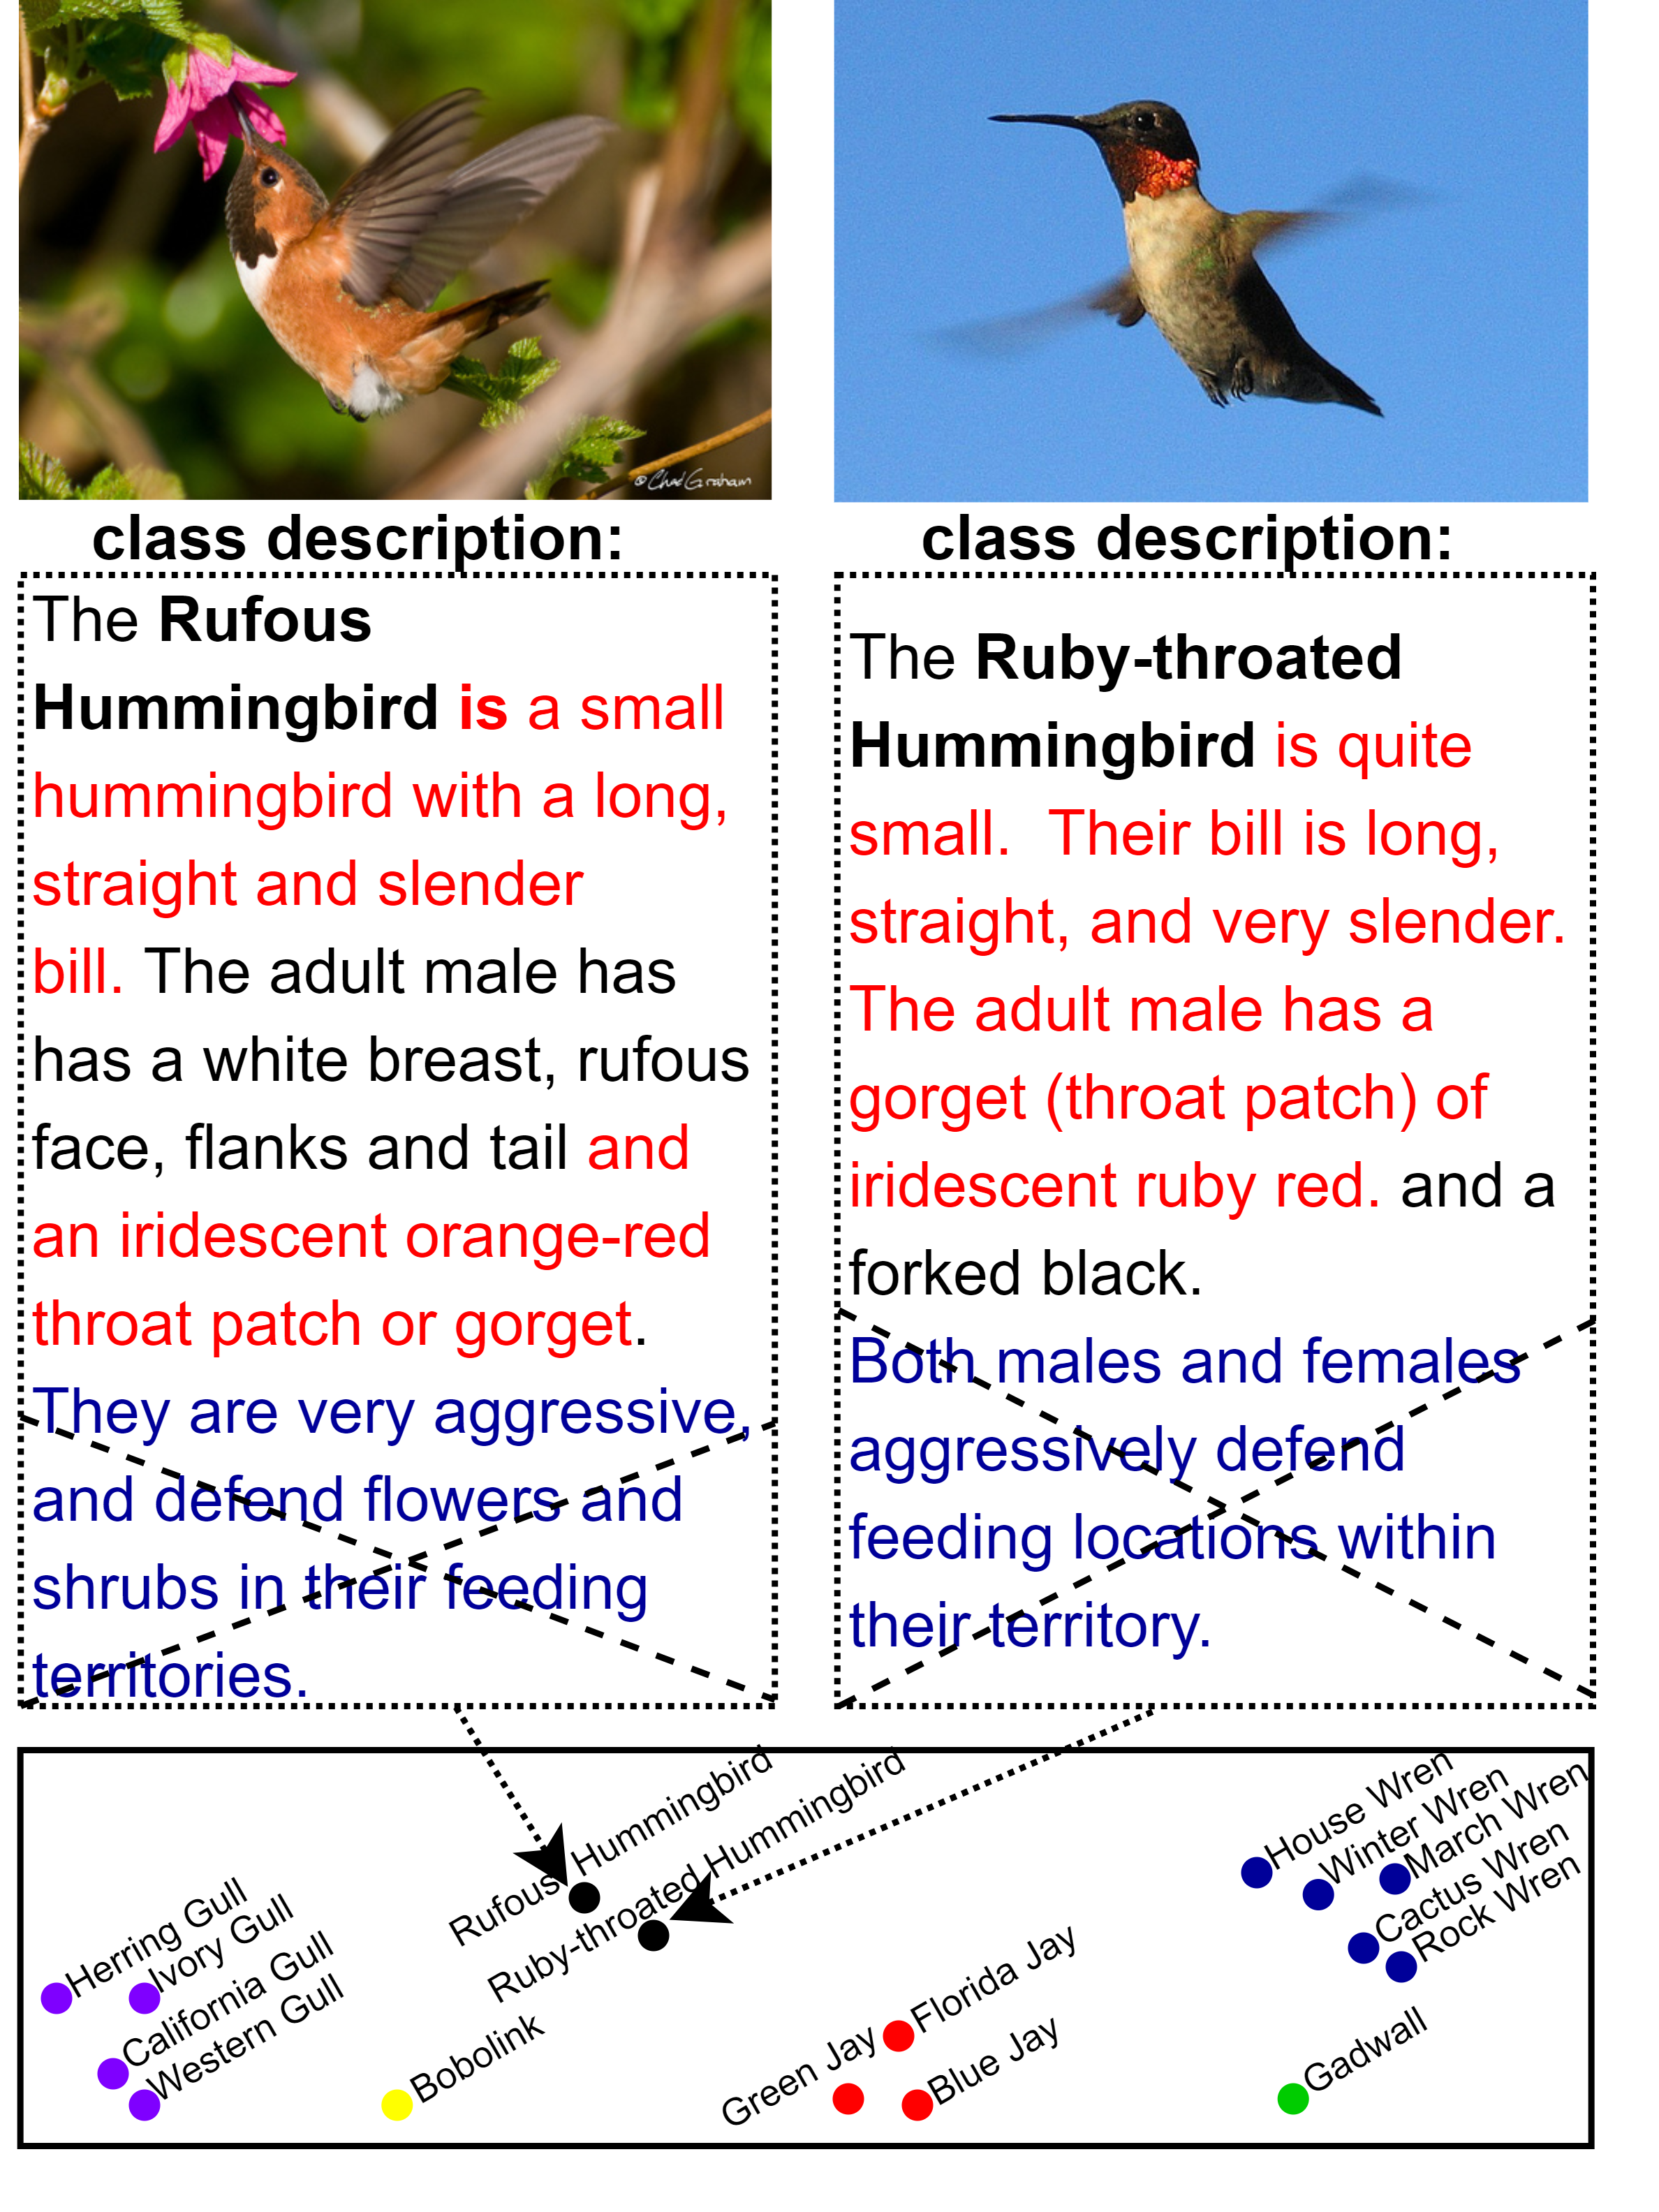
\includegraphics[width=\textwidth]{images/ZEST_text_similarities_differences_2 (6).png}}
 \caption{Textual similarity and visually relevant-descriptions enhancing: (1) Our approach leverages the similarity within %\gal{visually-relevant} \tzuf{no}
 texts (red) via document clustering (bottom box);
 % - representing documents clustered and labeled alphabetically
 %\gal{clustering of what?};
 (2) non-visually relevant description are removed (blue text) leaving both similar (red) and dissimilar (black) descriptions which are visually relevant. \yuval{Do we know which sentences DBSCAN uses for clustering, or red colors is just an illustration? We should be explicit on that.} 
 %\gal{ and what about the black text?}\tzuf{the black text shows differences.}
 }\ %\gal{Clarify in the figure that the text is class description, not image description. Clarify what  A,B<C stands for, Clarify what is the space in which the letters are located.}}
\label{fig:bird_example}%
\end{figure}

%A common setup for ZSL assumes that the auxiliary information is a set of semantically meaningful properties (called attributes) for describing the class (e.g., black-beak, long-tail) \citep{farhadi2009describing,lampert2009learning,changpinyo2020classifier,atzmon2018probabilistic}. Typically, these attributes are  manually collected by human raters for each image (test and train alike) and averaged across images. Another setup for ZSL use image-captions as the auxiliary information \citep{reed2016learning,Felix_2018_ECCV, Xian_2018_CVPR,Sariyildiz_2019_CVPR}. The captions are collected over test images, and a class description is an averaged embedding of hundreds or thousands of captions. 
%%
%The class description is then produced by averaging scores per attribute in all images that belong to the class \gal{not necessarily}. 
%This process is problematic, as the human raters are exposed to images from the test-set --- which defeats the very  purpose of the ZSL setup. \gal{I'm not sure that you want to attack everyone in the field on the 2nd paragraph} \tzuf{wasn't this Yuval's point which you agreed upon?}
%\citep{farhadi2009describing, lampert2009learning, atzmon2018probabilistic,akata2013label,wang2013unified,changpinyo2016synthesized, akata2015label,ji2018stacked}. \par


A common setup for ZSL assumes that the auxiliary information is a set of semantically meaningful properties (called attributes) for describing the class (e.g., black-beak, long-tail) \citep{wah2011caltech,farhadi2009describing,lampert2009learning,changpinyo2020classifier,atzmon2018probabilistic}. Another setup for ZSL uses hundreds or thousands of image-captions as the auxiliary information \citep{reed2016learning,Felix_2018_ECCV, Xian_2018_CVPR,Sariyildiz_2019_CVPR}. Typically, these auxiliary information are  manually collected by human raters for each image (test and train alike) and averaged across images.
%. The captions are collected over test images, and a class description is an averaged embedding of hundreds or thousands of captions. 
A more realistic approach 
relies on available online text that describes classes (e.g., wikipedia) \cite{elhoseiny2017link}. It thus avoids the expensive annotation and exposure to images from the test-set. The input of the task is now (1) an image; and (2) the text descriptions of the classes. 

%\gal{Here you want to explain the main challenges in from wiki descriptions: That most of the text is irrelevant to bird appearance, and only a few sentences are relevant.}

In this work we classify bird species according to wiki-like descriptions.
This task raises many challenges: 
(1) Differences between the birds are very small, which makes ours a very fine-grained classification task; (2) This is an expert task, %as in addition to the small difference between the birds, the 
and the text contains terminology that is unlikely to be familiar to a layman; and, on top of that
(3) The text descriptions of the classes are long, containing few visually relevant sentences. 
%(3) The text descriptions of the classes are long and very noisy.
Moreover, one can address this ZSL  task in two scenarios: %The ZSL task contains two real scenarios:
(i) an \enquote{easy} scenario, where  a new unknown object that is similar to  previously seen objects; (2) a \enquote{hard} scenario, where the new object is very different from seen one, i.e., belonging to a different family or species than those observed during training.

%thus, the relevance between seen and unseen objects is minimal.\par

As opposed to previous work,  here we focus on the {\em text} representation, and address a key question in ZSL, namely, how can we detect aspects of the text which would be important for classifying images? that is, \textit {how can we identify text components that are visual in nature?}
%%%%The key idea is to leverage the similarities between the seen and unseen classes, and identify salient visually-relevant information in the previously-unseen classes descriptions.  %Thus, in an easy scenario where the horse is known to us but the zebra is not - we can benefit from the similarity between the objects and texts. Whereas in a hard scenario we know neither the class of horses or zebras, and we want to classify a new image as horse or zebra. This requires that we enhance the visual differences in the text.\par


%To get an intuition on the task, 
%\gal{(1) This feels out of place. Either move    to earlier paragraph or move to later  when you explain the idea of similarity and embedding.  } \tzuf{Reut and I have been back and forth on the position of this paragraph. I don't see else where it can belong and it is important as people from NLP just don't get this task.}
To get an intuition about the task setup and our proposed solution, consider the following situation.
Imagine you never saw a zebra in your life but know how a horse looks like. What if you were given a text describing a zebra: \enquote{Zebras have hooves, mane, tail, pointed ears, and white and black stripes}. This description would probably be very close to a description of a horse having \enquote{hooves, mane, tail, pointed ears} and you would probably be looking for an image that reminds you of a horse but has \enquote{white and black stripes}. So, even without ever seeing a zebra, using text-descriptions of the zebra and  knowledge already acquired on horses, one can correctly classify unknown categories like a zebra.

%which aspects of the text are important for classifying images?
Our proposed solution is, likewise, two-phased. First,
based on the intuition that similar objects (or images thereof) tend to have similar texts,  %create a kernel-like method \gal{I think this is not kernel-like after all}  \reut{edited. how's that?} 
we encode a similarity feature that  enhances the separability of  text descriptions. %that reflects real similarity of the objects; 
In addition, we leverage the intuition that the differences between species would be their most salient visual features, and extract visually relevant  descriptions from the text.
%thus enhancing the compatibility of the text and the image ( Figure \ref{fig:bird_example}). 



Our experiments empirically demonstrate both the {\em efficacy} and  {\em generalization} capacity of our proposed solution. 
In experiments carried out on two large ZSL datasets, %\reut{(cite cub and nabirds)}, %\gal{not exactly}
in both the {\em easy} and {\em hard} scenarios, the similarity method obtains a ratio improvement of up to 18.3\%. With the addition of extracting visually relevant descriptions, we obtain a ratio improvement of up to 48.16\% over the state-of-the-art.
%Furthermore, we show the generality of our 
We further show that our visual-summerization method generalizes across datasets, and we demonstrate its contribution to additional models by a ratio improvement of up to 59.62\%.



%Our main contributions are as follows:  
The contributions of this paper are thus three-fold.
%\begin{enumerate} \item 
First,  to the best of our knowledge we are the first to show-case the critical importance of the text representation in zero-shot image-recognition scenarios, and we present two concrete text-based processing methods that vastly improve the results.
Secondly, we demonstrate the efficacy and generalizability of our proposed methods by applying them to both the {\em zero-shot} and {\em generalized zero-shot} tasks, outpreforming all previously reported results on the CUB and NAB Benchmarks \reut{ref,ref}. Finally, we show that visual aspects learned from one dataset can transfer effectively  to another dataset without the need to obtain dataset-specific annotations.  
%\end{enumerate}
The efficacy of our proposed solution on a variety of models and datasets illustrates that purposefully exposing the {\em visual features in texts} is indispensable  for tasks which learn to align the  vision-and-language modalities. %\gal{revise.}\reut{Edited. check if agree?}


\section{Background and Related Work}
\yuval{Relate to caption-based ZSL (Reed 2016 and following works)} \tzuf{already in the introduction}
%Recent successes of deep learning methods for the task of object recognition are heavily dependent on large dataset collection.
%Moreover, the number of categories keeps increasing and with it the need to collect more data. However, this process of collecting millions of images and their corresponding tags is highly expensive and time-consuming. \par
%\reut{I suggest adding the related work to the end (right before the conclusions) as customary in NLP papers, in order to not break our storyline}
Zero-shot learning (ZSL) %--- that is, learning to classifying images to descriptions based on a set of image-description pairs disjoint of those appearing at test time ---  
aims at overcoming the need to label massive datasets for new categories, by learning the connections between images and prior auxiliary knowledge about their classes. At test-time, this auxiliary information compensates for the lack of previously-attained visual information about  the new categories.
%Thus, the input is an image and auxiliary information about the classes, and the output is the class label. In the zero-shot phase, new classes are given, unseen during training. In the ZSL, the auxiliary information's function is to compensate for the unseen-before visual information.
%%
%%
Text-based ZSL is a specific multimodal instantiation of this learning task. Models for ZSL are typically composed of three parts: (1) the text representation (2) the image-representation (3) a compatibility function between the two modalities: image and text.   While most previous work focused mainly on the latter two components, here we %\cite{zhu2018generative, akata2015evaluation}. In this work we 
focus on the text.  

Most ZSL  studies   for object recognition are aimed at processing  the image modality. This holds for studies as \citet{xu2018attngan,lei2015predicting,qiao2016less,akata2016multi}, that rely on visual features  extracted using the well-established method of
Convolutional Neural Network (CNN) \cite{lecun1995convolutional}. More recent studies use object detection methods to detect the {\em semantic parts} of the object, and extract visual features at the part-level \cite{elhoseiny2017link,zhu2018generative,zhang2016spda}. This
method makes the image more compatible with the text, as it enables text-terms such as \enquote{crest} to be linked to the visual representation of parts like \enquote{head}. 



%There are different approaches as to the function that learns compatibility function between images and their textual descriptions: (1) \textbf{Visual-to-Semantics:} learning a function that maps from the visual space to the semantic space \citep{socher2013zero}. Thus, if one has an image, the function predicts the correct text related $F(X)=Y$ where X is the images and Y the texts; (2) \textbf{Semantics-to-Visual:} learning a function from the semantic space to the visual space \citet{zhu2018generative} $F(Y)=X$. This can be done by generating images from text, thus, the problem becomes a \enquote*{regular} classification problem as we now have generated images with the corresponding text labels; (3) \textbf{Joint learning:} simultaneously learns a function from the semantic and visual space to a common space and predicts a compatibility score: $F(X,Y)=score$  \cite{akata2015evaluation,akata2016multi,qiao2016less,elhoseiny2013write,elhoseiny2016write}.\par






ZSL studies to date that rely on textual descriptions  often rely on impoverished  text representations, such as Bag-of-Words (BOW) and Term Frequency-Inverse Document Frequency (TF-IDF), and focus on improving the visual representation and the model \cite{lei2015predicting,elhoseiny2013write,elhoseiny2016write,elhoseiny2017link,zhu2018generative}. Beyond that,  \citet{qiao2016less} used a simple BOW and a l2,1-norm based objective function to suppress the noisy signal in the text. However, this impoverished treatment of the text  is problematic, as it contains crucial information for detecting the correct class. 

In this work we proceed in  a different yet complementary direction to previous work, aiming to purposefully  model the contribution of the textual modality to the ZSL classification.
%{\em compatibility} function that is aimed to to learned between textual and visual modality --- a compatibility  that can then be effectively detected in an end-to-end  architecture. 
%This line of work proceeds after and {\em complements} the work done on the visual modality.
%At a more high-level view, our goal is to 
We aim to establish the importance of adequately processing the text into a sound representation of  visually salient features, in order to  increase the vision-and-language compatibility, that can then be effectively learned in an end-to-end manner.

%\section{Zero-shot Learning (ZSL) Background}

\section{Vanilla ZSL Baseline Models}
\label{task}

The key idea underlying our proposed solution is to transform the text representation from a non-task-oriented text representation to a task-oriented representation focusing on the most salient features for the visual recognition task. \yuval{It was hard for me to parse this sentence}
%%
Concretely, instead of letting the text representation encode a broad class-description, we designed a representation that encodes specifically the {\em similarities} and {\em differences} from other species. 

To do so, we employ two different (complementary) methods: (i)  inducing a similarity cluster; and (ii)  extracting visually relevant text descriptions. Both methods are incorporated in our proposed end-to-end vision-and-language classification architecture, presented in Figure~\ref{fig:model}. In what follows, we described our basic architecture (3.1), the similarity component (3.2), and the extraction of visually relevant summaries (3.3).


\begin{figure*}[th]
\centering
\scalebox{1}{
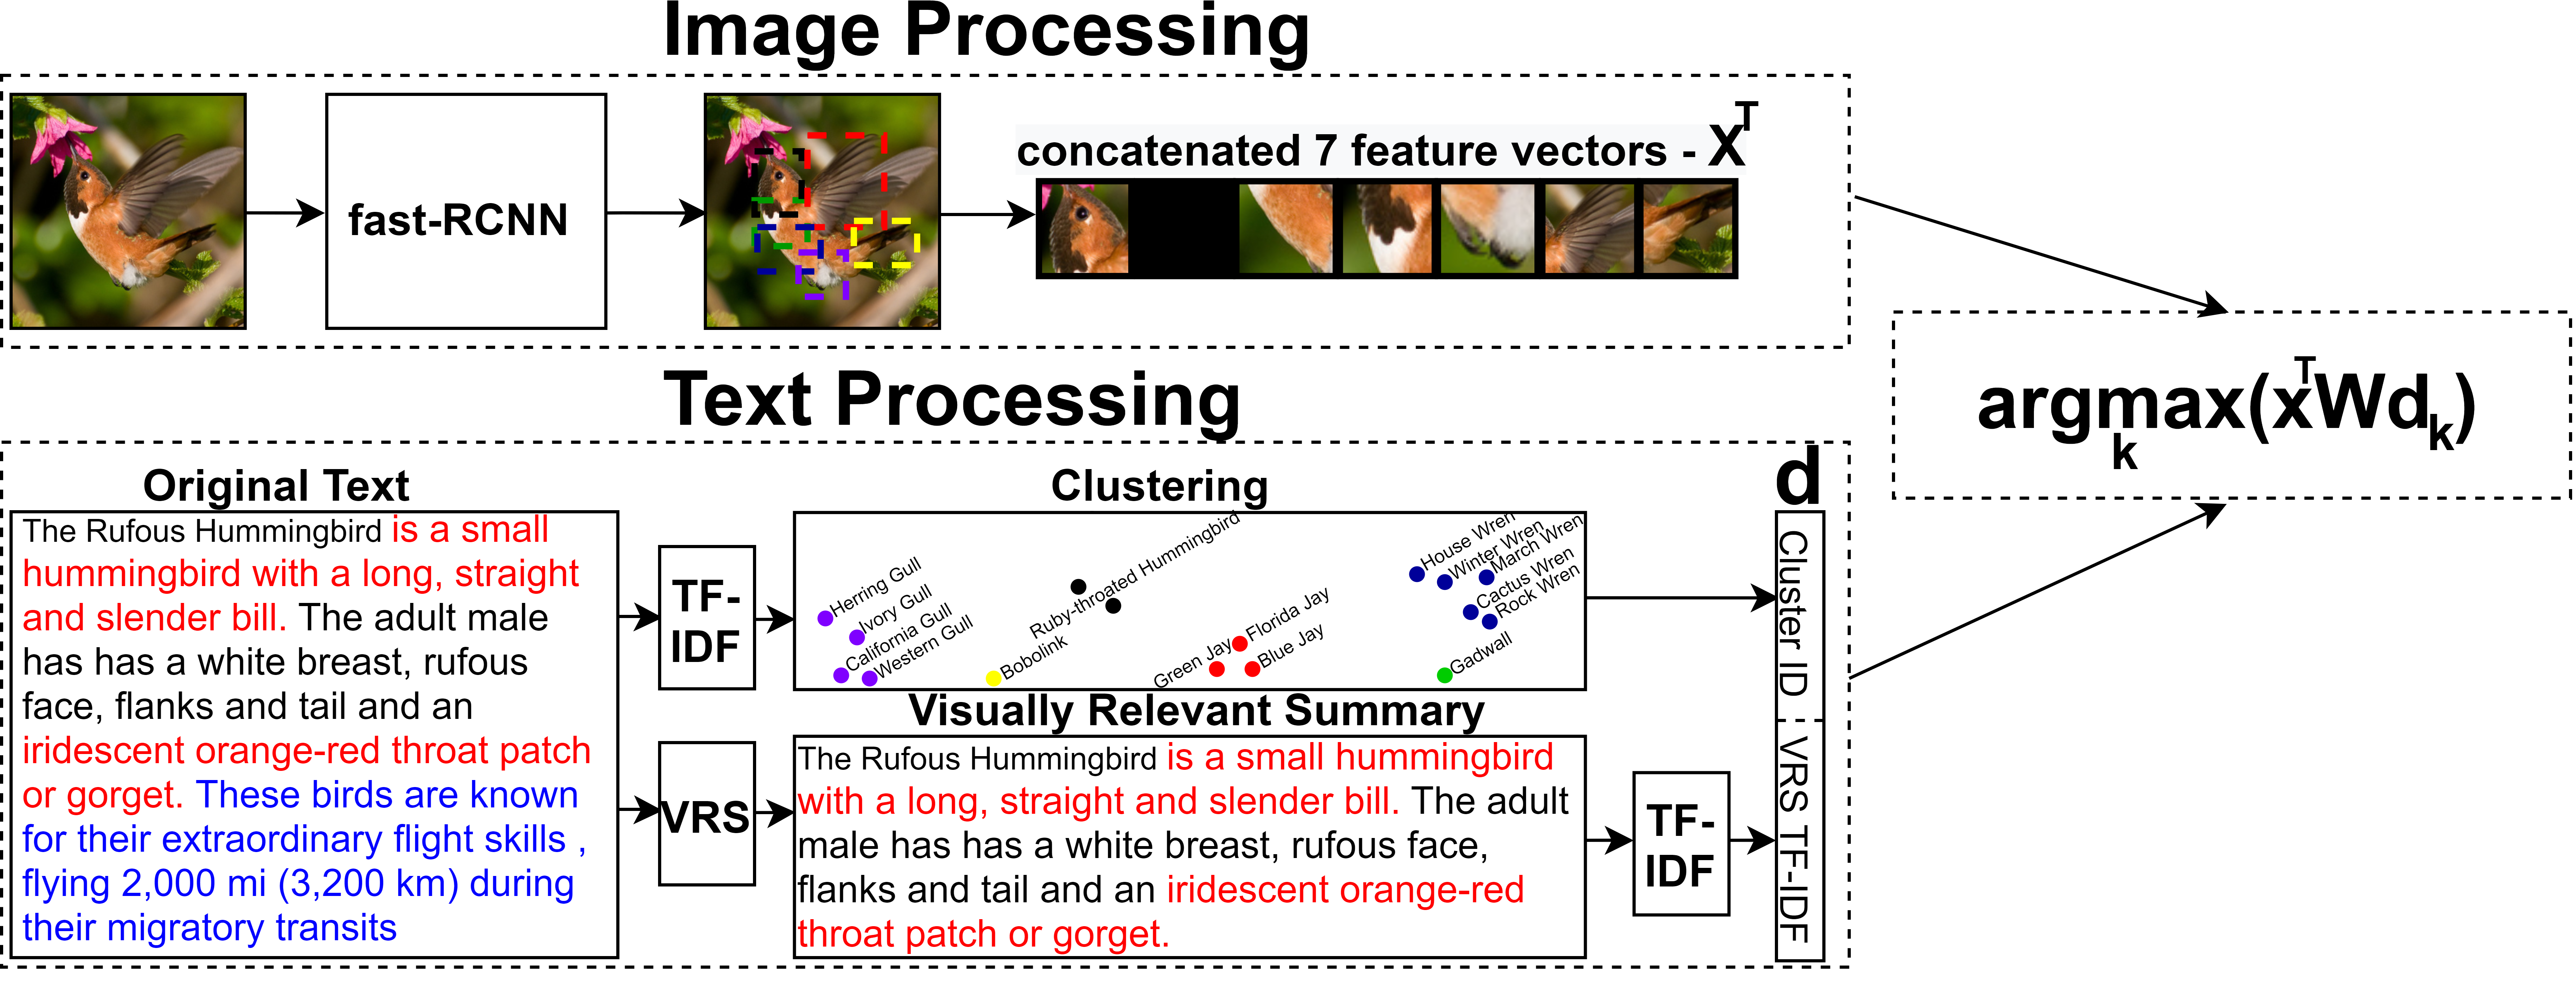
\includegraphics[width=\textwidth]{images/ZEST_model12.png}}
 \caption{Our ZEST$_{similarity}$+VRS model with the similarity and Visually Relevant Summaries (VRS).}
\label{fig:model}
\end{figure*}
\subsection{Basic Architecture (ZEST$_{vanilla}$)}
\yuval{I wouldn't call this ZEST$_{vanilla}$, or say it is ``ours''. People have already used linear compatibility+CE loss as baselines. What about just calling it \textit{Vanilla} or \textit{VanillaCE}}

Our basic {\em vanilla} architecture is a simple multiplicative attention mechanism \cite{luong2015effective} inspired by \citet{romera2015embarrassingly}. We model the problem using an attention-based model, where the image is queried
%considered 
against a set of candidate documents.

Formally, let $x^{\mathcal{S}}_1,\ldots,x^{\mathcal{S}}_{|S|}$ be the image feature vectors from a training-set, where $x^{\mathcal{S}}_i\in \mathbb{R}^{m}$. The set of training images corresponds to a set of $|\hat{S}|$ \textbf{seen} classes. Each class has a \textit{single} \enquote{class description} which is a document written by experts in free language (e.g.  wikipedia). We denote  $d^{\mathcal{S}}_1,\ldots,d^{\mathcal{S}}_{|\hat{S}|}$ as the sets of  document feature vectors, 
where $x^{\mathcal{S}}_i\in \mathbb{R}^{\hat{m}}$.
Likewise, $x^{\mathcal{U}}_1,\ldots,x^{\mathcal{U}}_{|U|}$ be the image feature vectors from a test-set, where $x^{\mathcal{U}}_i\in \mathbb{R}^{m}$. The set of test images corresponds to a set of $|\hat{U}|$ \textbf{unseen} classes. Each class has a \textit{single} \enquote{class description} which is a document written by experts in free language (e.g.  wikipedia). We denote  $d^{\mathcal{U}}_1,\ldots,d^{\mathcal{U}}_{|\hat{U}|}$ as the sets of  document feature vectors, 
where $x^{\mathcal{U}}_i\in \mathbb{R}^{\hat{m}}$.




%of size   $|S|$ and  $x^{\mathcal{U}}_1,\ldots,x^{z}_{N^{z}}$ be the image  vectors from a   zero-shot set ``$z$'' of size $N^{z}$. All image vectors are of dimensionality   $x^{t}_i,x^{z}_i\in \mathbb{R}^{m}$.
%\gal{A set would be a good idea. You can remove the definition of $D$ as a matrix.}
%Likewise, let $d^{t}_1,\ldots,d^{t}_{\hat{N}^{t}}$ and $d^{z}_1,\ldots,d^{z}_{\hat{N}^{z}}$ be sets of  document feature vectors in the  training set and zero-shot set, of size $\hat{N}^{t}$ and  $\hat{N}^{z}$,  respectively, where $d^{t}_i,d^{z}_i\in \mathbb{R}^{\hat{m}}$.

%\yuval{I would replace $t$ by $\mathcal{S}$, $\hat{N}^{t}$ by $|S|$ (seen), $z$ by $\mathcal{U}$ $\hat{N}^{z}$ by $|U|$ (unseen) and say explicitly that these are the number on classes, and that each class has a \textit{single} ``class description'', which is a document written by experts in free language (e.g.  wikipedia)}
%$d_1,\ldots,d_{\hat{N}}$, $d\in \mathbb{R}^{{m'}}$ be a set of $m'$ document feature vectors, each for another class. Let 
%Finally,  \(W\in  \mathbb{R}^{m\times\hat{m}}\) is our parameters matrix to be learned from the data. At inference time, given a test instance ${x_i}^{z}$ we select the label with the largest dot-product through the matrix $W$. The inferred label is:
\begin{equation}
    \label{equation:attention}
    {\hat{y}}=\argmax_{k} \left( x^{\mathcal{U}} \right) ^{T}Wd^{\mathcal{U}}_{k}, k = 1 : \hat{|U|}
\end{equation}
\gal{k maximization should be over the number of classes, not the number of images.}

For an image representation $x^{\mathcal{S}}_i$ and a text representation $d^{\mathcal{S}}_j$, an indicator function $I(x^{\mathcal{S}}_i,d^{\mathcal{S}}_j)$  outputs 1 if image $x^{\mathcal{S}}_i$ corresponds to the class described by $d^{\mathcal{S}}_j$ and 0 otherwise. 
The matrix $W$ is then learned by minimizing the categorical cross-entropy loss: 
\begin{equation}
\begin{split}
    %&\mathcal{L(W)}= \\
    \frac{1}{|S|}\sum_{i=1}^{|S|}\sum_{j=1}^{|\hat{S}|}I(x^{\mathcal{S}}_i,d^{\mathcal{S}}_j) 
    &\times\log(\textit{softmax}({x^{\mathcal{S}}_i}^TWd^{\mathcal{S}}_j))
\end{split}
\end{equation}

%\gal{this doesnt make sense. learning or inference? Define the inference problem first, and then define the learning problem.}


%Where $d\in D$ is the document in the set of documents $D$ that receives the maximum score on the dot product with $x$. 



\begin{figure}[t]
\centering
\scalebox{0.42}{
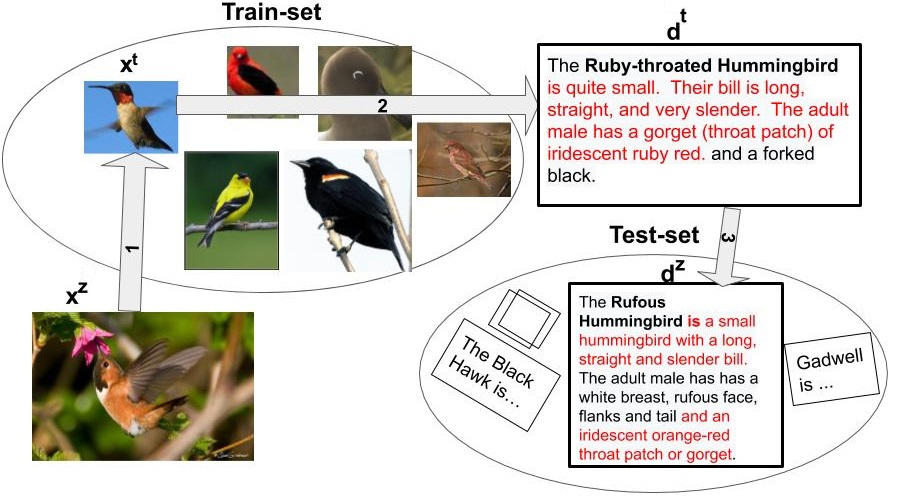
\includegraphics[width=\textwidth]{images/DS_model3.jpg}}
 \caption{Deterministic Similarity (DS) model}
\label{fig:DS}
\end{figure}

\subsubsection{Image Encoder}
\label{section:Image_Encoder}
The goal of the visual encoder is to transform the image to a vector representation of the most salient visual features for the classification. 

We adopt the image encoder for text-based ZSL of \citet{zhang2016spda, zhu2018generative,elhoseiny2017link}. It is based on Fast Region-based Convolutional Network framework (Fast R-CNN with VGG16 backbone) for object detection \citep{girshick2015fast} to detect seven semantic parts in the CUB dataset:
\enquote{head},\enquote{back},\enquote{belly},\enquote{breast},\enquote{leg},\enquote{wing},\enquote{tail}. 
. The encoded features of each visual part are then concatenated into a feature vector which functions as the image representation for the text-based ZSL.


% We adopt a 
% Fast Region-based Convolutional Network framework (Fast R-CNN) for object detection   \citep{girshick2015fast} to detect seven semantic parts in the CUB dataset:
% \enquote{head},\enquote{back},\enquote{belly},\enquote{breast},\enquote{leg},\enquote{wing},\enquote{tail}. 
% This image-representation method was present by \citet{zhang2016spda} and applied to the text-based ZSL task \cite{zhu2018generative,elhoseiny2017link}.
% %%
% The images are first encoded by VGG16 architecture \citep{simonyan2014very} and then visual features are extracted from parts detected using Region of Interest Pooling pooling (ROI) layer \citep{girshick2015fast}. %add cite to ROI pooling
% The encoded features of each visual part are then concatenated into a feature vector which functions as the image representation for the text-based ZSL.


\subsubsection{Basic Text Encoder}
\label{section:Text_Encoder}
Our basic encoder processes the text into a feature vector. Similar to previous studies, we employ a Term Frequency-Inverse Document Frequency (TF-IDF)  representation \citep{salton1988term}. %which requires the following pre-processing:
We pre-process the text to tokenize the words, remove stop words, and stem the remaining words. Then we extract of a feature vector using TF-IDF. This processing procedure is similar to the text processing presented by \citet{zhu2018generative}.
The dimensionalities of TF-IDF features for CUB and NAB are 7551 and 13217 respectively. 


\subsection{The Importance of being Similar}
\yuval{I would revise both titles saying ``the importance of XX''. Can we say something more explicit about the claim of this section? Currently it is confusing, since it is not clear who is ``being'' similar, how do we measure importance? do we measure importance at all? how do we use this importance, etc.. }

Our first proposed method leverages the similarities between images and texts. Meaning, when the actual classes of the images look similar, the texts are also similar,
%Similarities between texts reflect on real similarities between objects, 
and we want to reconstruct this analogy-like link. \yuval{(1) It was hard for me to parse this sentence. (2) Not suggest to not use the word analogy. It is reserved for a different set of works.}


%The TF-IDF representation of texts is at the word-level, representing the uniqueness of a word in the document and across documents. However, this word-level similarity fails to take more high-level document-level similarities into account.  
%%
%%
%Our intuition is that similarities between texts will suggest a similarity between objects, and vice versa.
%%
 To this end, we propose two models: (1) a deterministic model (2) adding a similarity component to our stochastic model ZEST$_{vanilla}$.
%%
For both models we use the Image Encoder (section \ref{section:Image_Encoder} to process the images $x$, and the Text Encoder (section \ref{section:Text_Encoder}) to process documents D.

\subsubsection{Deterministic Similarity (DS) Model}
\yuval{(1) Since it is a baseline, I would shorten this to a single paragraph and put it under the experiments section. Because it cuts the flow of the paper, it is not compatible with the vanilla method and it is not clear how it is related to the vanilla method. (2) maybe it is better to call it a cosine-similarity nearest-neighbour baseline. }

%Our approach leverages the analogy between images and texts. 
Figure \ref{fig:DS} presents our Deterministic Similarity (DS) method, that aims to  reconstruct  the parallel similarity links (a.k.a., analogies) between the  vision and text latent spaces. 

%Let  $x^{zero}$  represent a previously-unseen image in the zero-shot phase, and let \(x^{train}_k\) denote the $k$ image in a set of $N^{train}$ images from training.
%image of label \(k \in 1:N\) from the set of labels seen in the training set. 
%Likewise, \(d^{train}_{k}\)  (and \(d^{zero}_{k}\)) denote the description  of a seen (unseen) image with $\hat{N}^{train}$ and $\hat{N}^{zero}$ size sets in the training (and zero-shot) phase respectively.\par

The algorithm is as follows. Given an image $x^z_i$ in the zero-shot phase,
we first look for the image in the set of training images that is most similar to $x^z_i$. To do so we calculate the cosine similarity between $x^z_i$  and all the images from the training-set $x^{t}_k, k=1:N^{t}$.
where $\cos$ denotes the cosine similarity.
%%
%cosine similarity between  and all the images from the training-set $x^{train}_k, k=1:N$. 
\begin{equation}
{k}^*= \operatorname*{argmax}_{k}\cos(x_i^{z},x^{t}_k), k = 1:N^{t}
\end{equation}
Image $x_{k^*}^{t}$ is now the image that had received the highest cosine-similarity score. Next, we look for the training  document corresponding to that image. Here $f$ is simply a function that maps  a training image $x_i^{t}$ to its corresponding training document.
\begin{equation}
d^{t}_{k^*}=f(x^{t}_{k^*}) 
\end{equation}
Now \(d^{t}_{k^*}\) is the description of a bird-image that is most similar to \(x_i^{z}\). From the set of all documents in the zero-shot phase, we seek the document that is the most similar to $d_{k^*}^{t}$.
We again use
 the cosine similarity, between $d_{k^*}^{t}$ and any of  the texts in the zero-shot set $d^{z}_k, k = 1 : \hat{N}^{z}$.
 %, where $d^{zero}_k$ is a  document in the zero-shot set  \(k\in 1:\hat{N}\).
 The class label  $\hat{y}$ is thus the predicted category for the input image $x^{z}_i$.
 %of possible class descriptions.
\begin{equation}
\hat{y}= \operatorname*{argmax}_{k}\cos(d^{t}_{k^*},d^{z}_{k}), k = 1 : \hat{N}^{z}
\end{equation}


%\gal{A general repeated comment.
%All variables should be clearly defined before used. The way argmax is used throughout this paper seems wrong to me. Please 
%do not remove this comment until the issues are fully fixed. }

%
%\gal{The maximization domain of the argmax does not make sense. Did you mean to max of k? write the domain (the space you maximize over) explicitly.}
%



%\gal{Why the weird $<>$ notation for dot product? What do you mean by the norm over matrix $\| D^{zero}\|$. Did you mean to define a cosine similarity?  if so then (a) you dont need to, (b) this definition is incorrect.}

\section{Proposed Approach}
\subsection{ZEST$_{similarity}$}
\yuval{This is a major novelty of this work, I would explain it in more detail, }
%Having established the importance of similarity, \reut{have we really already eastablished that?} here 
A different way to incorporate textual similarity into the classification is to embed it into our stochastic model ZEST$_{vanilla}$, to benefit from it in the learning procedure. %Our approach aims to transform the text space into a linearly separable space, where sets of texts of similar species are separable.  \yuval{wouldn't go there}


The Basic Encoder used captures similarities and differences at the word-level. However, to find similarities at the document level we add to this vector our $similarity$ component \yuval{What is this component? First time it is described. Give more detail. }, which applies unsupervised clustering to  all class decsriptions in the training and test texts.   

This similarity-based representation is thus the TF-IDF vector concatenated with its cluster index, and it is then passed as  input to the ZEST$_{vanilla}$ architecture described in Section~\ref{section_ZEST_C}.  
%%
We hypothesize that the similarity component will work well on the \enquote{easy} scenario - where closely related birds are seen during training,  and their text can cluster together to indicate these similarities.

\subsection{The Importance of Being Seen}

Here we extract visually relevant features \textit{from the text}, making the texts that enters the classification more compatible with the salient visual information typically reflected in images. 

While the similarity method takes advantage of the similarity between objects seen in training and objects seen at test time, here we want to address the harder scenario, where similar objects are observed together during test time only (e.g. zebras and mules), and they may be very different from those observed during training.  

To differentiate between  classes in the test-set we need to emphasize the parts that are  different, both in the image and the text --- and these are typically their most salient visual features. % Our aim here is then to extract  visually relevant features from the text, thus making the texts that enters the classification more compatible with the salient visual information typically reflected in images. % Yuval: I moved this the last sentence to the opening of this section 


 
\subsubsection{Visually Relevant Summaries (VRS)}

%\gal{No hyphenation of compund adjectives when it has an 'ly suffix'. See rules of using hyphens www.grammarbook.com/punctuation/hyphens.asp} 

Our method for enhancing the textual description is based on visually relevant extractive Summaries.
Extractive summarization is the task of extracting a small number of sentences that summarize a given document.
In this work we define {\em visually relevant extractive summarization} (VRS) as the task of extracting only sentences which represent {visually relevant} language. The term {\em visually relevant language} (VRL) was coined by \citet{winn2016detecting} to indicate sentences which are visually descriptive with respect to the object (i.e., bird species).


A {na\"{i}ve} approach for VRS would be to extract sentences with  parts that we know are visually salient in our domain (e.g., the 7 parts employed by the vision recognition representation).  However, this na\"{i}ve approach has the several drawbacks. First, bird parts can be described using many different terms and paraphrases; additionally, a bird can be described by its property values (e.g. black), without any mention of the  attribute (e.g.,  beak). 
Instead, we propose to use the similarity of sentences in the wiki to naturally occurring sentences  (`in the wild') containing VRL descriptions. % According to this approach, if we want to extract sentences that contain VRL than we need to compare the similarity between sentences in the document and other VRL sentences 

Note that we cannot rely on descriptions of particular species due to the zero-shot setup. We must do with descriptions of objects in the  {\em  general kind} %that can be  be obtained for the {\em general class} 
of objects we are interested in classifying. 

\subsubsection{ZEST$_{similarity}$+VRS}
One way to obtain naturally-occurring descriptions of birds is from captions that describe bird images. Critically, these captions need {\em not}  be from  our dataset, they can describe any bird image. 

We propose to use a set of bird captions to create an unsupervised classifier that predicts whether a sentence is relevant, that is, whether it contains descriptions that can be {\em seen} in a bird image.
%We use only captions of birds that are seen during training.

For each document we propose to calculate the pairwise similarity between captions and sentences in the wiki-description, and based on this similarity, assign a VRS-score to each sentence.

% To this end, we embed both captions ($c_{0:L}$) and sentences ($s_{0:M}$) in the document using
% pre-trained BERT network  \cite{devlin2019bert}. The output encoded-tokens are then passed to a pre-trained siamese and triplet networks \citep{Schroff_2015_CVPR} to derive semantically meaningful fixed-size sentence embeddings that can be compared using cosine-similarity \citet{reimers2019sentence}.
% The VRS-score of sentence $s_j$ with respect to all available captions   $c_{1:L}$  is thus defined to be:


We calculate the VRS-score of a sentence $s_j$ to a caption by computing the cosine similarity of the embedding of both the captions ($c_{0:L}$) and sentences ($s_{0:M}$) in the document. For a fixed-size sentence embeddings, we use a pre-trained siamese-and-triplet network \citep{reimers2019sentence, Schroff_2015_CVPR} on top of a pre-trained BERT network  \cite{devlin2019bert}.

% The output encoded-tokens are then passed to a pre-trained siamese and triplet networks \citep{Schroff_2015_CVPR} to derive semantically meaningful fixed-size sentence embeddings that can be compared using cosine-similarity \citet{reimers2019sentence}.

The VRS-score of sentence $s_j$ with respect to all available captions   $c_{1:L}$  is thus defined to be:


\begin{equation}
\begin{aligned}
\begin{split}
\label{eq:score}
&score(s_j)=  \frac{1}{L}
&\sum_{i=0}^{L} \frac{c_i\cdot s_j}{\| s_j\|\| c_i\| }
\end{split}
\end{aligned}
\end{equation}
\gal{looks like you wanted to define an average over cosine scores $\sum_i\cos(c_i, s_j)$. We already used cosine before, no need to define it now. }


We then take the highest scoring  30 sentences from \(s_{0:M}\) (or $\frac{3}{4}M$ sentences in the document, whichever is lower) \gal{30 and 3/4 looks arbitrary. Are you certain that you did not look at the test set when you selected this? you need to show the sensitivity of the results to these values. Also, I recommend that you write here that you take the top $k$, and in the experiment section write that you used $k=30$} to be the visually relevant extractive summary of the document. We can then concatenate the similarity embedding to the VRS summary of the text, and perform the multiplicative attention on the this  revised encoding of the documents and the same image encoding as before.\par
\yuval{Why 30 sentences? or 3/4? Did we choose it on a validation set? Is it a common rule of thumb?}

A bird's eye 
%(pun intended)
overview of our overall architecture is presented in Figure~\ref{fig:model}.
%\reut{I had to :) feel free to remove the pun but leave the ref to the table}. 
Note that the text that enters the $similarity$  (clustering) component is the original wiki document, {\em not} the VRS summary of the document. Documents contain many non-visual descriptions that are unobserved in the images. However, these non-visual descriptions might still be important to capture the similarity between the documents (e.g. similar-looking birds are likely to be in the same habitat). Thus, the VRL sentence extraction and the similarity enhancement are performed in parallel on the original document. 
\section{Experiments}

\subsection{Experiment setting}

\paragraph{Datasets:}  We evaluate our method on the Caltech UCSD Birds-2011 dataset (CUB) \citet{wah2011caltech} and the North America’s birds dataset (NAB) \cite{van2015building}, using class descriptions obtained from wikipedia and the AllaboutBirds website \cite{AllaboutBirds}, collected by \citet{elhoseiny2017link}. 
Both are datasets of birds, with small differences in the images and texts, making it a challenging task of fine-grained classification. The CUB dataset contains 11,788 images of 200 bird species, and the NAB
is a larger dataset of birds with 48,562 images of 404 classes\footnote{\citet{elhoseiny2017link} merged the original 1,011 classes according to the subtle division of classes.}.
In addition, the texts of both CUB and NAB are long, containing a lot of non-visual information. CUB has an average of 869 tokens and 42 sentences in class documents. NAB has an average of 1277 tokens and 58 sentences in class documents. 

\paragraph{Two split Settings} We use the two splits for both datasets presented by \citet{elhoseiny2017link}: (1) Super Category-Shared (SCS), also referred to as the \enquote*{easy} split; and (2) Super-Category-Exclusive (SCE), also referred to as the \enquote*{hard} split. In the SCS-split, for each class in the test-set, at least one class in the training set belongs to the same category (categories are organized taxonomically). E.g. in Figure \ref{fig:bird_example}, the Rufous Hummingbird and the Ruby-throated Hummingbird are both from the Hummingbird category. In the SCE-split scenario, all the classes in a category are in the same set, such that, if a class is in the test-set then other classes from the same category will only be in the test-set, and will never be seen during training. Intuitively, classes from the same category have high similarity in both images and texts, so while in the SCS-split similar images have been seen during training, in the SCE-split a class from an entitrely new category is seen for the very first time. %but a very similar looking bird was seen in training, making it easier than the SCS.

\paragraph{Clustering Algorithms:}
The parameters of our model include clusters parameters.
We use two clusters methods: (1) Density-based spatial clustering of applications with noise (DBSCAN) \citep{ester1996density}; (2) Hierarchical DBSCAN \citep{mcinnes2017hdbscan}.
We optimize the parameters on a validation set \gal{which parameters?}. All variants of the ZEST model are trained using categorical cross-entropy. \yuval{Describe the details of the validation set. Unless we used the same set as Elhoseiny or others. Then just say we use their val set.}
%optimization loss

\paragraph{Human Summarization:} 
To evaluate our proposed VRS extraction method, we designed an oracle experiment using ground-truth visually relevant summarization. To this end, we manually annotated the CUB dataset by extracting sentences which include visually relevant descriptions of the bird subject. On average, only 11.9\% of the sentences were found to include VLR.  

\paragraph{Image Captions:}
To create visual summaries we use image captions of birds from the CUB train-set, provided by \citet{reed2016learning}.  Each image in the CUB dataset has been annotated with 10 fine-grained captions. These captions describe only the visual appearance of the birds while avoiding mentioning the name of the bird specie. E.g., \enquote{This bird has a long beak, a creamy breast, and body, with brown wings}. In this work we use the first 5 captions of each image.


To showcase the generality of this approach, we use these captions in both in-domain (CUB) and out-of-domain (NAB) scenarios. In all cases we avoid using captions of unseen (test) bird classes.  In the latter case we effectively use captions from CUB to extract VRS for entirely-different species in represented in NAB.  Note that {\em only} models that include the VRS component (+VRS) employ these image captions. We report learning curves to indicate the amount of captions that are realistically needed.



%We limit the use of caption to those that correspond to  mages that are seen during training in the CUB dataset. In the NABirds all caption from the CUB dataset are allowed.


\paragraph{Baselines:}  
Our approach is compared asainst ten leading algorithms (see Table \ref{tab:results}): MCZSL \citep{akata2016multi}, WAC-Linear  \citep{elhoseiny2013write}, Wac-Kernel   \citep{elhoseiny2016write}, ESZSL     \citep{romera2015embarrassingly}, SJE   \citep{akata2015evaluation}, Sync$_{fast}$ \citep{changpinyo2016synthesized}, Sync$_{OVO}$ \citep{changpinyo2016synthesized},
ZSLNS \citep{qiao2016less}, and GAZSL \citep{zhu2018generative}. 


\paragraph{Generalized Zero-Shot Learning:} 
The conventional zero-shot learning task considers only unseen classes during zero-shot phase. However, in a realistic scenario seen objects might also appear \cite{chao2016empirical}. In Generalized Zero-Shot Learning (GZSL), test data might also come from seen classes, and the labeling space is the union of both types of seen and unseen classes. GZSL is thus considered a more formidable problem setting
than ZSL due to the model's bias towards the seen classes.
%%
We follow the metric present by \citet{chao2016empirical} to evaluate our models on the GZSL task. We evaluate the accuracy of a Seen-Unseen accuracy Curve (SUC) and use Area Under  SUC to measure the general capability of ZSL methods.

 \begin{table}[t]
  \centering
 \scalebox{0.6}{

\begin{tabular}{l|ll|ll} 
\Xhline{6\arrayrulewidth}
\multirow{2}{*}{\textbf{ methods} }                                  & \multicolumn{2}{c|}{\textbf{CUB } }                                    & \multicolumn{2}{c}{\textbf{NAB} }                                     \\ 
\cline{2-5}
                                                                     & \multicolumn{1}{c}{\textbf{SCS} } & \multicolumn{1}{c|}{\textbf{SCE} } & \multicolumn{1}{c}{\textbf{SCS} } & \multicolumn{1}{c}{\textbf{SCE} }  \\ 
\hline
Random classification                                                          & 2                                 & 2.5                                & 1.23                              & 1.23                               \\ 
\hline
MCZSL \citet{akata2016multi}                        & 34.7                              & -                                  & -                                 & -                                  \\
WAC-Linear \citet{elhoseiny2013write}          & 27.0                              & 5.0                                & -                                 & -                                  \\
WAC-Kernel \citet{elhoseiny2016write}              & 33.5                              & 7.7                                & 11.4                              & 6.0                                \\
ESZSL \citet{romera2015embarrassingly}              & 28.5                              & 7.4                                & 24.3                              & 6.3                                \\
SJE \citet{akata2015evaluation}                    & 29.9                              & -                                  & -                                 & -                                  \\
ZSLNS \citet{qiao2016less}                          & 29.1                              & 7.3                                & 24.5                              & 6.8                                \\
SynC$_{fast}$ \citet{changpinyo2016synthesized}     & 28.0                              & 8.6                                & 18.4                              & 3.8                                \\
SynC$_{OVO}$ \citet{changpinyo2016synthesized}      & 12.5                              & 5.9                                & -                                 & -                                  \\
ZSLPP \citet{elhoseiny2017link}                   & 37.2                              & 9.7                                & 30.3                              & 8.1                                \\
GAZSL \citet{zhu2018generative}                   & 43.7                              & 10.3                               & 35.6                              & 8.6                                \\ 
\hline
Deterministic Similarity (DS) & 40.402                            & 5.551                              & 37.002                            & 5.517                              \\
ZEST$_{vanilla}$                                                                 & 39.16                            & 11.77                             & 27.61                            & 10.18                             \\
\textbf{ZEST$_{similarity}$}                                           & \textbf{47.48}                   & \textbf{11.77}                     & \textbf{38.2}                   & \textbf{10.18}                    \\
\hline
\textbf{ZEST$_{similarity}$+VRS}                                        & \textbf{48.57}                    & \textbf{15.26}                    & \textbf{38.51 }                   & \textbf{10.23 }                    \\ 
\Xhline{6\arrayrulewidth}
                 
\end{tabular}
}
\caption{Top-1 accuracy (\%) on CUB and NAB datasets with two split settings.}
\label{tab:results}
\end{table}


\begin{table}[t]
\centering
 \scalebox{0.61}{
\begin{tabular}{l|cc|cc} 
\Xhline{6\arrayrulewidth}
\multirow{2}{*}{\textbf{ methods} } & \multicolumn{2}{c|}{\textbf{CUB } }                                                              & \multicolumn{2}{c}{\textbf{NAB} }           \\ 
\cline{2-5}
                                    & \textbf{SCS}                                    & \textbf{SCE}                                   & \textbf{SCS}         & \textbf{SCE}          \\ 
\hline
GAZSL                               & \begin{tabular}[c]{@{}c@{}}43.74\\\end{tabular} & \begin{tabular}[c]{@{}c@{}}10.3\\\end{tabular} & 35.6                 & 8.6                   \\
GAZSL+parts summarization                               & \begin{tabular}[c]{@{}c@{}}19.54\\\end{tabular} & \begin{tabular}[c]{@{}c@{}}9.557\\\end{tabular} & 23.32
                 & 7.2
                   \\
GAZSL+parts summarization +${similarity}$                               & \begin{tabular}[c]{@{}c@{}}38.25\\\end{tabular} & \begin{tabular}[c]{@{}c@{}}9.557\\\end{tabular} & 33.05
                 & 7.2
                   \\
GAZSL+our VRS                            & 43.72                                           & \textbf{16.44}                                       & 37.28
                & 9.237                 \\
GAZSL+HUMAN                         & 35.98                                           & 21.81                                          & -                    & -                     \\
GAZSL+HUMAN+${similarity}$                       & 47.32                                           & 21.81                                          & -                    & -                     \\ 
\hline
            ZEST$_{vanilla}$                                                                 & 39.16                            & 11.77                             & 27.61                            & 10.18                             \\
                
                 
  ZEST$_{vanilla}$+our VRS                             & {42.58}                                  & {15.26}                                 & {32.24}      & {10.23}        \\
ZEST$_{similarity}$                                & 47.48                                           & 11.77                                          & 38.2
                & 10.18                 \\
ZEST$_{similarity}$+parts summarization                                & 42.27
                                           & 10.93
                                          & 37.02

                & 8.055
                 \\
ZEST$_{similarity}$+ our VRS                             & \textbf{48.57}                                  & {15.26}                                 & \textbf{38.51}      & \textbf{10.23}        \\

ZEST$_{similarity}$+HUMAN                          & 48.99                                & 17.2                                           & -                    & -                     \\ 
\Xhline{6\arrayrulewidth}
\end{tabular}
}
    \caption{Visually Relevant Summarization (VRS) with GAZSL, ZEST$_{vanilla}$, and ZEST$_{similarity}$.  }%
    \label{table:summarization}%
\end{table}





\begin{table}[t]
\centering
 \scalebox{0.87}{
\begin{tabular}{l|c|c} 
\Xhline{6\arrayrulewidth}
    \multirow{2}{*}{ \textbf{methods }} & \textbf{CUB }  & \textbf{NAB }   \\ 
\cline{2-3}
                                    & \textbf{SCS }  & \textbf{SCS}   \\ 
\hline
ZEST$_{vanilla}$                     & 39.16          & 27.61          \\
ZEST$_{vanilla}$ + bird category  & 43.71          & 36.73           \\
Zest$_{similarity}$ only 1 cluster             & 46.55          & 35.94           \\
Zest$_{similarity}$ full (2 cluster) & \textbf{47.48} & \textbf{38.2}   \\
\Xhline{6\arrayrulewidth}
\end{tabular}
}
    \caption{Zest model with different similarity methods}%
    \label{table:similarity}%
\end{table}




\begin{table}[t]
\centering
 \scalebox{0.76}{
\begin{tabular}{l|cc|cc} 
\Xhline{6\arrayrulewidth}
                  \multirow{2}{*}{\textbf{ methods} } & \multicolumn{2}{c|}{\textbf{CUB } }                                                              & \multicolumn{2}{c}{\textbf{NAB} }           \\ 
\cline{2-5}
                                    & \textbf{SCS}                                    & \textbf{SCE}                                   & \textbf{SCS}         & \textbf{SCE}          \\ 
\hline
ESZSL             & 0.185           & 0.045             & 0.092           & 0.029             \\
ZSLNS             & 0.147           & 0.044             & 0.093           & 0.023             \\
WAC$_{kernal}$         & 0.225           & 0.054             & 0.007           & 0.023             \\
WAC$_{linear}$         & 0.239           & 0.049             & 0.235           & -                 \\
SynC$_{fast}$          & 0.131           & 0.040             & 0.027           & 0.008             \\
SynC$_{OvO}$           & 0.017           & 0.010             & 0.001           & -                 \\
ZSLPP             & 0.304           & 0.061             & 0.126           & 0.035             \\
GAZSL             & 0.354           & 0.087             & 0.204           & 0.058             \\ 
\hline
ZEST$_{similarity}$              & \textbf{0.443 } & \textbf{0.1 }     & \textbf{0.267 } & \textbf{0.067 }   \\
\hline
ZEST$_{similarity}$+VRS           & \textbf{0.437}           & \textbf{0.147}             & \textbf{0.26}            & \textbf{0.084}             \\
ZEST$_{similarity}$+HUMAN        & 0.445           & 0.163             & -               & -                 \\
\Xhline{6\arrayrulewidth}
\end{tabular}
}
    \caption{Generalized Zero-Shot Learning: AUC of Seen-Unseen Curve.}%
    \label{table:GZSL}%
\end{table}


\subsection{Results}
Table \ref{tab:results} presents the top-1 accuracy for each of the models. 
The table is divided into four sections, which are (from top to bottom): 
(1) random classification; (2) previous work; (3) our models with previous setup (for comparison to previous work); (4) Our model with additional data - captions. 

\paragraph{DS Model:} 
According to table \ref{tab:results}, the DS model achieves competitive results on the SCS-split - 40.402\% and 37.002\% on CUB and NAB correspondingly. The high scores on the SCS-split, where similar birds have been seen during training, is expected --- as this method relies on similarities within texts and images. 
%
In contrast, the DS suffers from low accuracy on the hard-split, where different categories of birds have been seen  during training. As the DS model relies on text and image similarities, it is intuitively appealing that low accuracy on the SCE stems from the fact that birds from different categories are less likely to look alike. 

\paragraph{ZEST$_{vanilla}$}
In contrast to the very sophisticated approaches of \citet{zhu2018generative}, our simple stochastic text-based approach \yuval{I wouldn't call $ZEST_{vanilla}$ ``ours''. Maybe say ``the vanilla cross-entropy based approach''} outperforms all previous methods on the SCE-split on both CUB (+14.27\% ratio of improvement) and NAB (+18.37\%  ratio of improvement). As the SCE-split is a more challenging split, this sheds light on the strength as well as limitations of this simple framework.  

\paragraph{ZEST$_{similarity}$}

Next we embed the similarity approach inspired by the DS model into the stochastic system. %obtaining combined strengths over both the SCE and SCS splits.
\yuval{I suggets to revise. IIUC, DS does not learn anything. and the similarity index was obtained from the clustering models.  }
The ZEST$_{similarity}$ model adds the similarity to the representation of the text-only if over 15\% of the texts from test-set are clustered with at least one text from train-set we concatenate the encoded cluster label to the document representation $d$. \yuval{Describe this under the approach. Also explain how the 15\% thershold was chosen.}
Thus, in the case of the SCE-split no or few similarities are found, and the ZEST$_{similarity}$ preforms at the same level as the ZEST$_{vanilla}$ model. 

%The combination of a simple yet strong framework as the ZEST$_{vanilla}$ and the similarity addition achieves state-of-the-art on all split, in both CUB and NAB datasets. \reut{Do we  need this paragraph?}


The two clustering algorithms we applied find real similarities, achieving high accuracy when tested on predicting the correct label according to the ground-truth taxonomical category. The HDBSCAN, and DBSCAN achieved 88\% and 84.5\% accuracy on the CUB, and 93.07\% and 95.05\% on the NAB, accordingly.

Interestingly though, different clustering find different sources of similarities, that are essentially {\em additive}. In Table \ref{table:similarity} we can see a comparison between different similarity enhancing methods. 
The ZEST$_{vanilla}$ + bird category method is a BOW of the bird category added to the original text embedding and then passed as before to a ZEST$_{vanilla}$ model. 
The use of two clusters that capture different similarities (ZEST$_{similarity}$) improves our model over an embedding of the bird category (ZEST$_vanilla$ + bird category) in the text representation, by an absolute improvement of up to 3.77\%. This suggests that our $_{similarity}$ method captures similarities that are beyond the bird category. %(e.g, birds that are visually similar).  

Finally, 
in Table \ref{table:GZSL} we present the results of ZEST$_{similarity}$  the GZSL setup. On both datasets and splits, the ZEST$_{similarity}$ achieves the state-of-the-art with up to 30.88\% ratio improvement.

\paragraph{ ZEST$_{vanilla}$+VRS and ZEST$_{similarity}$+VRS }
%The ZEST$_{vanilla}$+VS and  ZEST$_{similarity}$+VS models
use the captions from training images in the CUB in order to generate visually relevant extractive summaries of the original wiki documents.

We test the summarized representation on the ZEST$_{vanilla}$ model, the ZEST$_{similarity}$ and the GAZSL \citep{zhu2018generative} model. In Table \ref{table:summarization} we show the experimental results. We compare the models before and after the use of the Visually Relevant  Extractive Summarization component. We see an improvement in accuracy in both models on both datasets and on both splits. The GAZSL improves especially on the SCE-split, as the similarity between texts is reduced. In contrast, the ZEST$_{similarity}$ with the similarity component handles the SCS-split, having a component that enhances the similarity in the text representation.  

In addition, we see a drop in the GAZSL+HUMAN performance on the SCS-split. This is because the summarization process of the text reduces the similarity which is important in the SCS-split. However, when adding our similarity model to the GAZSL+HUMAN --- GAZSL+HUMAN+$similarity$,  the performance goes up again.
\reut{the part about GAZSL and the  paragraph after need revision, message unclear.} 

To assess the quality of the VRS summarization performance we treat HUMAN summarization as the ground truth. The VRS method succeeds in removing 49.4\% of the sentences in on the CUB dataset with 96.23\% recall and 22.59\% precision. For comparison, removing 49.4\% of the sentences randomly produces a recall of 50.6\% and a precision of 11.9\%.
Another comparison we made is to a state-of-the-art extraction summarization model such as  Textrank \citep{mihalcea2004textrank} algorithm, which achieves a recall of 12.33\% and a precision of 12.83\%.

 
We then compare both ZEST$_{similarity}$ and the GAZSL to the use of HUMAN summarization in the CUB dataset and see additional improvement in both models on the two splits. The gap between the performance on the VRS and the Human summarization indicates that improvement in the summarization of documents will improve the models' performance, and is, therefore, a promising path for text-based zero-shot learning research.


\begin{figure}[t]
\centering
\scalebox{0.47}{
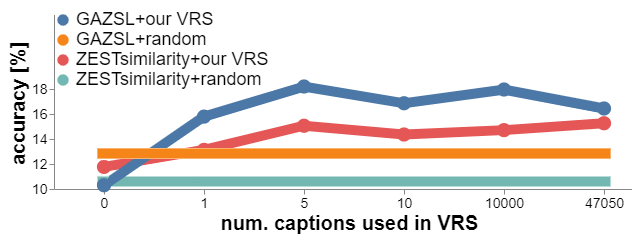
\includegraphics[width=\textwidth]{images/captopm_graph_5.png}}
 \caption{Accuracy per number of captions used to \textit{focus}   summarization, measured on the hard SCE split of CUB. Showing that as little as 5 captions in total are sufficient to focus the summarization process.
 %\yuval{(1) I would change the figure xlabel to ``num. captions used to \textit{focus}   summarization''. (2) The random baselines are still confusing. Could you make them  a single marker on the Y  y axis?}
 }
\label{fig:captions}
\end{figure}


Finally, we experiment to assess the  number of captions that is realistically needed for the VRS method. The results, presented in Table \ref{fig:captions}, show that only a few (~5)
 sentences (captions) from arbitrary birds are needed to achieve the maximum accuracy with this method.
Testing the VRS with 5 arbitrary captions from CUB dataset on the NAB dataset with SCS-split we achieved a 39.28\% accuracy. %Thus, we need not resort to in-domain crowd-sourcing
%Thus, the VRS method does not require the use of crowd-sourcing to produce image captions. 
For comparison, \citet{reed2016learning} showed that his model relies on at least 512 captions \textbf{per class} to achieve the same accuracy as using all the captions available per class, during test-time.


%\reut{is this the case for both CUB and NAB or only CUB? maybe the low number is needed only in the in-domain scenario and out of domain will need more captures?} 


\par



\section{Conclusion}
\label{conclusion}

This work aimed to establish a better way to represent the text to generally support text-based ZSL task. Our two orthogonal text-processing methods lead to significant improvements across models, splits, and data-sets, and illustrate that adequate text-processing methods is essential  in text-based ZSL tasks, or indeed, and are conjectured to be essential in any vision and language-based tasks. 
%We thus, recommend applying text-processing methods in future research which includes vision and language modalities.\reut{Not sure about the last sentence, it appears to  repeat the previous one}


\bibliography{emnlp2020}
\bibliographystyle{acl_natbib}
\end{document}
